\begin{quote}
	\textit{``If the chaos of the nineties reflects a radical shift in the paradigms of visual literacy, the final shift away from the Lascaux/Gutenberg tradition of a pre-holographic society, what should we expect from this newer technology, with his promise of discrete encoding and subsequent reconstruction of the full range of sensory perception?''}
\end{quote}
\hfill \textit{Burning Chrome, William Gibson}
\\
\\

%=========================================================================================================

\label{chapter-conclusions}

Alternate realities have fascinated mankind since early prehistory and with the advent of the computer and the smartphone we have seen the rise of many different categories of alternate reality that replace, augment, diminish and mix with our familiar real world to expand our capabilities, our understanding and our entertainment.

This thesis has introduced parallel reality as a new category of alternate reality that comprises two environments, one real and the other virtual, each complete unto itself and wherein the user may freely switch between them. The benefits that such a system imparts upon the user by granting them the ability to explore parallel real and virtual environments in tandem has been shown by developing a parallel reality platform, Mirrorshades, and applying it to a use case within the realm of cultural heritage, with evaluation of these studies leading to a number of best practices for future parallel reality endeavours.

\begin{figure}[h]
	\begin{center}
		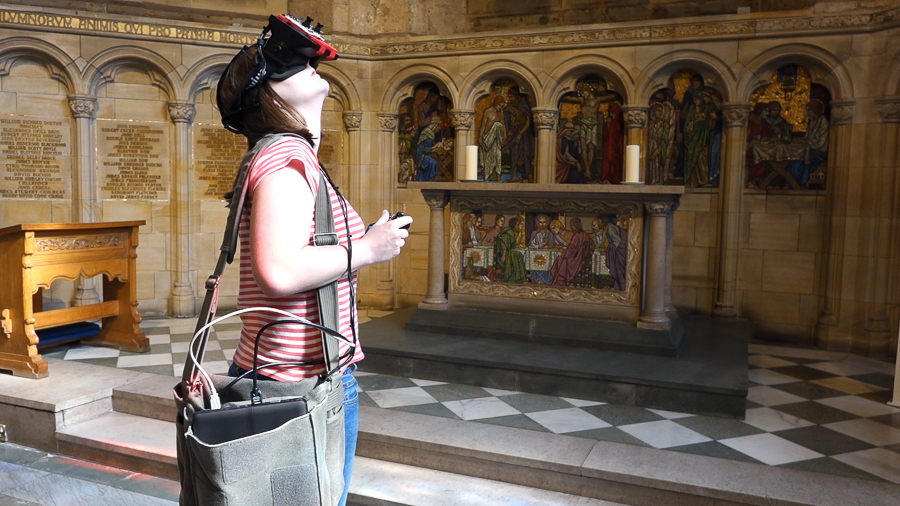
\includegraphics[width=\textwidth]{participant-f-4.jpg}
		\caption{The \textit{Mirrorshades} parallel reality platform in use.}
		\label{participant-f-4.jpg}
	\end{center}	
\end{figure}

%=========================================================================================================

\section{Contributions}

As listed in section \ref{intro-contributions} the contributions of this thesis can be summarized as follows;

\begin{itemize}
	\item The introduction of parallel reality as a new category of alternate reality that allows users to experience two complete environments in tandem and represents an approach for mitigation of the vacancy problem.
	\item The framing of parallel reality through a thorough investigation and extension of previous taxonomies that classify and distinguish alternate reality terminologies.
	\item The creation of the combined Milgram/Waterworth model for visualising alternate reality experiences, including those of parallel reality systems.
	\item Development of a parallel reality platform, dubbed Mirrorshades, that combines new virtual reality hardware with novel indoor positioning technology.
	\item Evaluation of the Mirrorshades platform through user studies of a real world use case study within the realm of cultural heritage, including the application of an established presence questionnaire to parallel reality.
	\item Discussion and creation of a set of best practices for future parallel reality endeavours.
\end{itemize}

%=========================================================================================================

\section{Future Work}

The introduction of parallel reality in this thesis along with the investigation of its first serious implementation in Mirrorshades is only the beginning of en extended course of study that will be required to fully understand \& come to appreciate the benefits that the concept can offer. The following highlights a few choice avenues in which the investigation into parallel reality would be well to pursue, but should be no means be considered an exhaustive list of possibly improvements \& extensions.

Probably most noticeable is the matter of hardware. The parallel reality platform presented by this thesis, Mirrorshades, is a somewhat cumbersome package of HMD, laptop, battery pack, smartphone, games console controller \& myriad cables, occupying both of the users hands \& requiring them to carry a satchel of not insubstantial size \& weight. To posit that this cumbersome nature of the platform had a directly detrimental effect upon the quality of experience received by the participants is no stretch of the imagination \& improvements in this regard will be required for parallel reality to see deployment \& use in anything but controlled laboratory or user study conditions. As discussed in section \ref{mobile-client} we are already beginning to see the advent of hardware platforms that would present a much improved basis for parallel reality experiences. A platform such as Samsung Gear VR, once appropriately modified with the requisite stereo video see-through provision, would represent a fully contained single unit parallel reality experience, suitable for handing to a user in the same manner that audio guides are given out at many of the world's museums. Furthermore, improvements to the performance of the platform, in terms of the visual acuity of both real \& virtual content, as well as the accuracy of the positioning \& registration, will present beneficial results both to casual users \& to experts wishing to use such a modality of interaction for serious work.

Investigating the application of parallel reality to other domains represents possibly the largest avenue of potential further extension. While the user studies discussed in this thesis experimentally showed the worth of parallel reality when applied to cultural heritage, parallel reality as a concept could be applied to many fields. Postulating for but a moment, one can imagine how parallel reality could be applied to architecture \& visualisation of renovations, using the physical layout of an environment as a canvas for novel artistic expression, to the study of PolySocial interactions involving real \& VR parties \& new styles of gaming that merge both real \& virtual play fields. As society becomes more familiar with \& more dependent upon almost constant connection to the virtual, whether in the form of 2D Web based social networks \& apps or richer multimedia experiences, the utility of platforms that allow real \& virtual environments to be cycled between in a trivial manner will likely present many exciting opportunities.

multiuser

Experience assessment


%=========================================================================================================

\section{Final Thoughts}

While the vision of Neil Stephenson's metaverse, where all computer mediated communication takes place within a persistent multi-user 3D virtual world, may still be many years to come, parallel reality has today already given us a glimpse into how mankind may one day integrate such a construct into their real environments in a manner akin to how the smartphone has for the 2D Web.

some success can be claimed



the words of Orlan (emphasis original);

\textit{``I come back therefore to my initial words about the `\textbf{and}' in order to propose the virtual \textbf{and} the real used simultaneously as new transversalities that question art and the becoming of our world.''}~\cite{Orlan2002}

%=========================================================================================================